\chapter{Mathematical Modelling and System Identification}
	
\section{Dynamic Flight Model}\label{SSECT_DynamicFLightModel}
\todo{Put in how the flight model in simulink works etc}
The dynamic flight model of the craft must cater for all six of the degrees of freedom the craft experiences. The dynamics of this system is modelled as of three rotational and three translational degrees of freedom \cite{Moller2015}. To continue deriving the equations of motion, the following assumptions are made: the aircraft is a rigid body, the aircraft has constant mass, $I_{xy}, I_{xz}, I_{yz}$ are all negligibly small.   

The Newton-Euler method of defining the accelerations uses the inertial frame to define the linear accelerations, and the body frame to define the rotational accelerations. Using Newton's first law and the rotation matrix described in \eqref{EQ_RotationMatrix}, the expression for the linear acceleration can be developed and is shown in \eqref{EQ_EulerNewtonInertialMatrix}.

\begin{equation}
\begin{bmatrix} \ddot{N}\\ \ddot{E}\\ \ddot{D} \end{bmatrix} = \begin{bmatrix} 0\\ 0\\ g \end{bmatrix} + \textbf{R} \begin{bmatrix} 0\\ 0\\ \frac{\textbf{T}}{m} \end{bmatrix}
\label{EQ_EulerNewtonInertialMatrix}
\end{equation}

The rotational accelerations of the craft can be similarly described using the moments and the simplified inertia tensor. These rotational rates are described in \eqref{EQ_EulerNewtonRotationMatrix}

\begin{equation}
\begin{bmatrix}\ddot{\phi}\\ \ddot{\theta} \\ \ddot{\psi} \end{bmatrix} = \frac{1}{\boldmath{I}} \times \begin{bmatrix} N  \\ M  \\ L \end{bmatrix} = \begin{bmatrix} I_{xx} N  \\ I_{yy} M  \\ I_{zz} L \end{bmatrix}
\label{EQ_EulerNewtonRotationMatrix}
\end{equation}
	
\section{System Identification}
In order to correctly model the system, a thorough system identification needs to be completed. This entails real world measurements of the chosen platform. The methods and results from these experiments are covered in this section.

	\subsection{Mass and Inertia}
	Using a calibrated scale the mass of the rotorcraft measured at 3.352Kg. To calculate moments of inertia, the Bifilar Pendulum method was used. The method is thoroughly described in literature and involves tying the drone from the ceiling allowing it rotate around one axis. Since it is desired to measure the inertias along three axes, three separate test set ups were required. Images of the test set up for a single axis is shown in \ref{IM_BifilarPendulum}. 
	
	\begin{figure}[H]
		\centering
		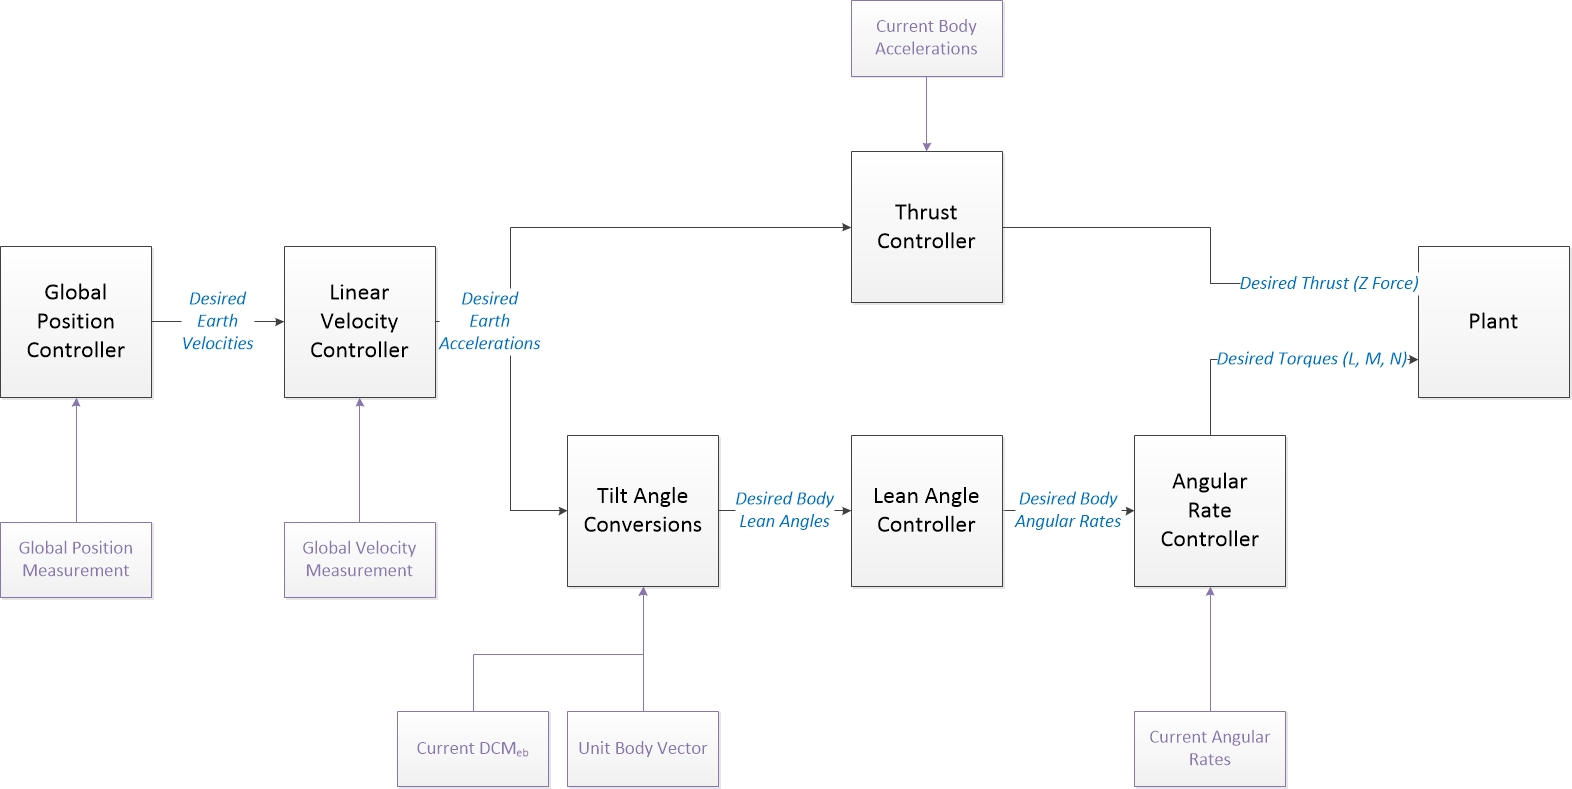
\includegraphics[height = 7.5cm]{../References/Diagrams/ControlDiagram.jpg}
		\caption{Bifilar Pendulum for Measurement}
		\label{IM_BifilarPendulum}
	\end{figure}
	
	Each axis was measured 10 times and the values were averaged out to obtain the final values represented in Table \ref{tab:MomentOfInertia}. To give a representation of measurement variance, the standard deviation is provided along side.
	
	\begin{table}[!]
		\centering
		\begin{tabular}{l | c | c | c |}
			Parameter & Averaged Measured Value & Standard Deviation\\
			\hline\hline
			$I_{xx}$ & 0.025027578 & 0.001063842\\
			$I_{yy}$ & 0.169260024 & 0.000142928\\
			$I_{zz}$ & 0.170196714 & 0.000527406\\
		\end{tabular}
		\label{tab:MomentOfInertia}
		\caption{Measured Moments of Inertia}
	\end{table}
	
	\subsection{Thrust and Moment Profiles}
	In order to correctly valid the thrust characteristics of the drone, each motor rotor pair needed to be evaluated. Each pair was marked and coupled to a load cell. The ESCs were configured to send varying PWMs to the motors. The commands sent to the ESCs and the measured thrust values are plotted together in Figure \ref{IM_ThrustProfiles}.
	
	\begin{figure}[H]
		\centering
		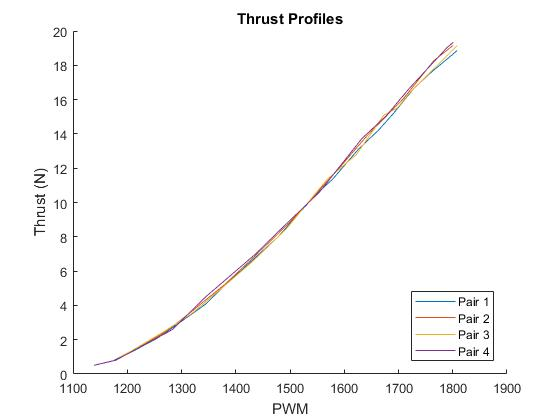
\includegraphics[height = 7.5cm]{../Design/Mechanical/ThrustProfiles/thrustprofiles.jpg}
		\caption{Bifilar Pendulum for Measurement}
		\label{IM_ThrustProfiles}
	\end{figure}
	
	\begin{table}[!]
		\centering
		\begin{tabular}{l | c | c | c |}
			Pair & Max Thrust & Min Thrust\\
			\hline\hline
			$1$ & 18.8558 & 0.7852\\
			$2$ & 19.1489 & 1.1889\\
			$3$ & 19.1434 & 0.9511\\
			$4$ & 19.3369 & 0.5087\\
		\end{tabular}
		\caption{Measured Moments of Inertia}
		\label{tab:ThrustProfiles}
	\end{table}
	
	\subsection{Drag Coefficients}
	\todo{How did you choose these?}
	
	\subsection{Sensor Constants}
	\todo{How did you choose these?}
		\subsubsection{Sensor Offsets}
		\todo{How did you choose these?}
		\subsubsection{Measurement Noise}
		\todo{How did you choose these?}
	\section{Instrumentation}
	\todo{Here is where you put how you created the instrumentation models and noise, based on what you learnt in the lit review}
	
	\section{Disturbances}
	\todo{Here is where you put how you created the disturbance models, based on what you learnt in the lit review}
	\subsection{Wind Model}
	\subsection{Drag Model}	
			
	\section{Discussion}
		